% TikZ-poster
% https://texdoc.net/texmf-dist/doc/latex/tikzposter/tikzposter.pdf
% https://www.overleaf.com/learn/latex/Posters
\documentclass[25pt, a0paper, portrait, innermargin=1.0cm, blockverticalspace=-5mm]{tikzposter}

\usepackage[utf8]{inputenc}
\usepackage{authblk}
\usepackage{url}
\usepackage{amsfonts, amsmath, amssymb, bm}
\usepackage{multicol}
\usepackage{caption}

% FONTS

\renewcommand{\familydefault}{\sfdefault}

% BIBLIOGRAPHY

\usepackage[backend=biber, style=nature]{biblatex}
\defbibheading{empty}{}
\DeclareFieldFormat{labelnumberwidth}{\mkbibbrackets{#1}}

\addbibresource{ref.bib}

% COLOURS
% https://latexcolor.com/

\definecolor{CaPink}{RGB}{232, 94, 138} % default pink
\definecolor{CaDarkUnsatPink}{RGB}{249, 26, 97} % dark unsaturated pink
\definecolor{CaLightPink}{RGB}{253, 175, 200} % light pink
\definecolor{CaRed}{RGB}{223, 47, 81} % red
\definecolor{cream}{rgb}{1.0, 0.99, 0.82} % cream

\colorlet{backgroundcolor}{white} % solid colour background
\colorlet{bgcolor}{cream!50!white} % gradient colour background
\colorlet{titlebgcolor}{white}
\colorlet{titlecolor}{CaRed}
\colorlet{framecolor}{black}
\colorlet{blockAtitlebgcolor}{CaPink}
\colorlet{blockBtitlebgcolor}{CaRed}
\colorlet{blockCtitlebgcolor}{CaLightPink}
\colorlet{blocktitlefgcolor}{white}

% TITLE STYLE

\definetitlestyle{sampletitle}{
width=780mm, roundedcorners=5pt, linewidth=10pt, innersep=5pt,
titletotopverticalspace=-6mm, titletoblockverticalspace=-5mm
}{
\begin{scope}[line width=\titlelinewidth, rounded corners=\titleroundedcorners]
% \draw[color=framecolor, fill=titlebgcolor]
% (\titleposleft,\titleposbottom) rectangle (\titleposright,\titlepostop);
\end{scope}
}

\settitle{ \centering \vbox{
\@titlegraphic \\[\TP@titlegraphictotitledistance] \centering
\color{titlefgcolor} {\bfseries \color{titlecolor} \Huge \fontsize{80}{80}\selectfont \@title \par}
\vspace*{1em}
{\@author \par} \vspace*{1em}
{\Large \@institute} % used for mail
\vspace*{1em}
}}
\renewcommand{\Authfont}{\bfseries\huge}
\renewcommand{\Affilfont}{\normalfont\Large}

\usetitlestyle{sampletitle}

% BLOCK STYLE(S)
% https://tex.stackexchange.com/questions/48756/tikz-relative-coordinates

\newcommand\titleoffset{-11mm}
\def\blocktitleheight{1.0cm}

\defineblockstyle{blockA}{titlewidthscale=0.9, bodywidthscale=1,titleleft,titleoffsetx=0pt, titleoffsety= \titleoffset, bodyoffsetx=0mm, bodyoffsety=0mm, bodyverticalshift=10mm, roundedcorners=5, titleinnersep=6mm, bodyinnersep=1cm}{\draw[color=blockAtitlebgcolor, fill=blockbodybgcolor,rounded corners=\blockroundedcorners,line width=2mm] (blockbody.south west) rectangle (blockbody.north east);\ifBlockHasTitle\draw[fill=blockAtitlebgcolor, color=blockAtitlebgcolor] ($ (blockbody.north west)!.1!(blockbody.north east) $) -- ($ ($ (blockbody.north west)!.2!(blockbody.north east) $) + (0, \blocktitleheight) $) -- ($ ($ (blockbody.north west)!.8!(blockbody.north east) $) + (0, \blocktitleheight) $) -- ($ (blockbody.north west)!.9!(blockbody.north east) $) -- ($ ($ (blockbody.north west)!.8!(blockbody.north east) $) + (0, -\blocktitleheight) $) -- ($ ($ (blockbody.north west)!.2!(blockbody.north east) $) + (0, -\blocktitleheight) $)  -- cycle;\fi
}
\providecommand\blockA[2]{{
\useblockstyle{blockA}
\block{\centering #1}{\selectfont#2}
}}

\defineblockstyle{blockB}{titlewidthscale=0.9, bodywidthscale=1,titleleft,titleoffsetx=0pt, titleoffsety= \titleoffset, bodyoffsetx=0mm, bodyoffsety=0mm, bodyverticalshift=10mm, roundedcorners=5, titleinnersep=6mm, bodyinnersep=1cm}{\draw[color=blockBtitlebgcolor, fill=blockbodybgcolor,rounded corners=\blockroundedcorners,line width=2mm] (blockbody.south west) rectangle (blockbody.north east);\ifBlockHasTitle\draw[fill=blockBtitlebgcolor, color=blockBtitlebgcolor] ($ ($ (blockbody.north west)!.02!(blockbody.north east) $) + (0, \blocktitleheight) $) -- ($ ($ (blockbody.north west)!.6!(blockbody.north east) $) + (0, \blocktitleheight) $) -- ($ (blockbody.north west)!.7!(blockbody.north east) $) -- ($ ($ (blockbody.north west)!.6!(blockbody.north east) $) + (0, -\blocktitleheight) $) -- ($ ($ (blockbody.north west)!.02!(blockbody.north east) $) + (0, -\blocktitleheight) $)  -- cycle;\fi
}
\providecommand\blockB[2]{{
\useblockstyle{blockB}
\block{#1}{#2}
}}

\defineblockstyle{blockC}{titlewidthscale=0.9, bodywidthscale=1,titleleft,titleoffsetx=0pt, titleoffsety= \titleoffset, bodyoffsetx=0mm, bodyoffsety=0mm, bodyverticalshift=10mm, roundedcorners=5, titleinnersep=6mm, bodyinnersep=1cm}{\draw[color=blockCtitlebgcolor, fill=blockbodybgcolor,rounded corners=\blockroundedcorners,line width=2mm] (blockbody.south west) rectangle (blockbody.north east);\ifBlockHasTitle\draw[fill=blockCtitlebgcolor, color=blockCtitlebgcolor] ($ ($ (blockbody.north west)!.98!(blockbody.north east) $) + (0, \blocktitleheight) $) -- ($ ($ (blockbody.north west)!.4!(blockbody.north east) $) + (0, \blocktitleheight) $) -- ($ (blockbody.north west)!.3!(blockbody.north east) $) -- ($ ($ (blockbody.north west)!.4!(blockbody.north east) $) + (0, -\blocktitleheight) $) -- ($ ($ (blockbody.north west)!.98!(blockbody.north east) $) + (0, -\blocktitleheight) $)  -- cycle;\fi
}
\providecommand\blockC[2]{{
\useblockstyle{blockC}
\block{\flushright #1}{#2}
}}

\defineblockstyle{blockBlank}{titlewidthscale=0.9, bodywidthscale=1,titleleft,titleoffsetx=0pt, titleoffsety= \titleoffset, bodyoffsetx=0mm, bodyoffsety=0mm, bodyverticalshift=10mm, roundedcorners=5, titleinnersep=6mm, bodyinnersep=1cm}
{
}
\providecommand\blockBlank[1]{{
\useblockstyle{blockBlank}
\block{}{#1}
}}

% SMALL TWEAKS

% remove watermark
\tikzposterlatexaffectionproofoff

% itemize item shape/color
\renewcommand\labelitemi{\color{CaRed}$\blacktriangleright$}

% custom caption
\captionsetup[figure]{labelfont={color=CaRed,bf},name={Fig.:},labelsep=none}
\renewcommand{\thefigure}{}

% column separation
\setlength{\columnsep}{1.5cm}
\setlength{\columnseprule}{0.1pt}

% affiliations
% https://tex.stackexchange.com/questions/352519/how-can-i-keep-multiple-authblk-affiliation-in-tikzposter-in-one-line
\makeatletter
\renewcommand\maketitle{\AB@maketitle} % revert \maketitle to its old definition
\renewcommand\AB@affilsepx{\quad\protect\Affilfont} % put affiliations into one line
\makeatother

\renewcommand\paragraph[1]{
\begin{center}
  {\bf\color{CaRed} #1}
\end{center}}

%%%%%%%%%%

% TITLE

\title{Collective motion in large deviations of active particles}

\author[1,2,3]{Y.-E. Keta}
\author[2,4]{\'E. Fodor}
\author[3]{F. van Wijland}
\author[2]{M. E. Cates}
\author[2,5]{R. L. Jack}

\affil[1]{Laboratoire Charles Coulomb, UMR 5221 CNRS, Universit\'e de Montpellier, France}
\affil[2]{Department of Applied Mathematics and Theoretical Physics, University of Cambridge,
Wilberforce Road, Cambridge CB3 0WA, United Kingdom}
\affil[3]{Universit\'e Paris Diderot, Laboratoire Mati\`ere et Syst\`emes Complexes,
UMR 7057 CNRS, F-75205 Paris, France}
\affil[4]{Department of Physics and Materials Science, University of Luxembourg, L-1511 Luxembourg}
\affil[5]{Department of Chemistry, University of Cambridge, Lensfield Road, Cambridge CB2 1EW, United Kingdom}

\institute{\url{yann-edwin.keta@umontpellier.fr}}

\begin{document}

% COLOUR GRADIENT BACKGROUND
% https://tex.stackexchange.com/questions/121000/adding-a-background-image-with-tikz-poster
% https://tex.stackexchange.com/questions/215895/color-gradient-in-tikzpicture-from-top-to-bottom-corner
\node[shading=axis, rectangle, left color=bgcolor, right color=bgcolor!30!white,shading angle=135, anchor=north, minimum width=\paperwidth, minimum height=\paperheight, above right,opacity=0.7,inner sep=0pt,outer sep=0pt] at (bottomleft){};
%%%%%%%%%%

\maketitle

\begin{columns}

\column{0.5}

\blockB{Motivation}
{
\begin{itemize}
  \item Large deviations of physical systems consider \textbf{transient rare events}, often accompanied by collective effects. Numerical techniques used to analyse these events enable us to study the \textbf{microscopic mechanisms which stabilise these atypical collective behaviours}.
  \item Some large deviations of isotropic active Brownian particles (ABPs) were shown to be associated with \textbf{collective motion} (CM), despite the \textbf{absence of any microscopic aligning interactions}. We study in greater details this transition to collective motion.\\
\end{itemize}

{
\centering
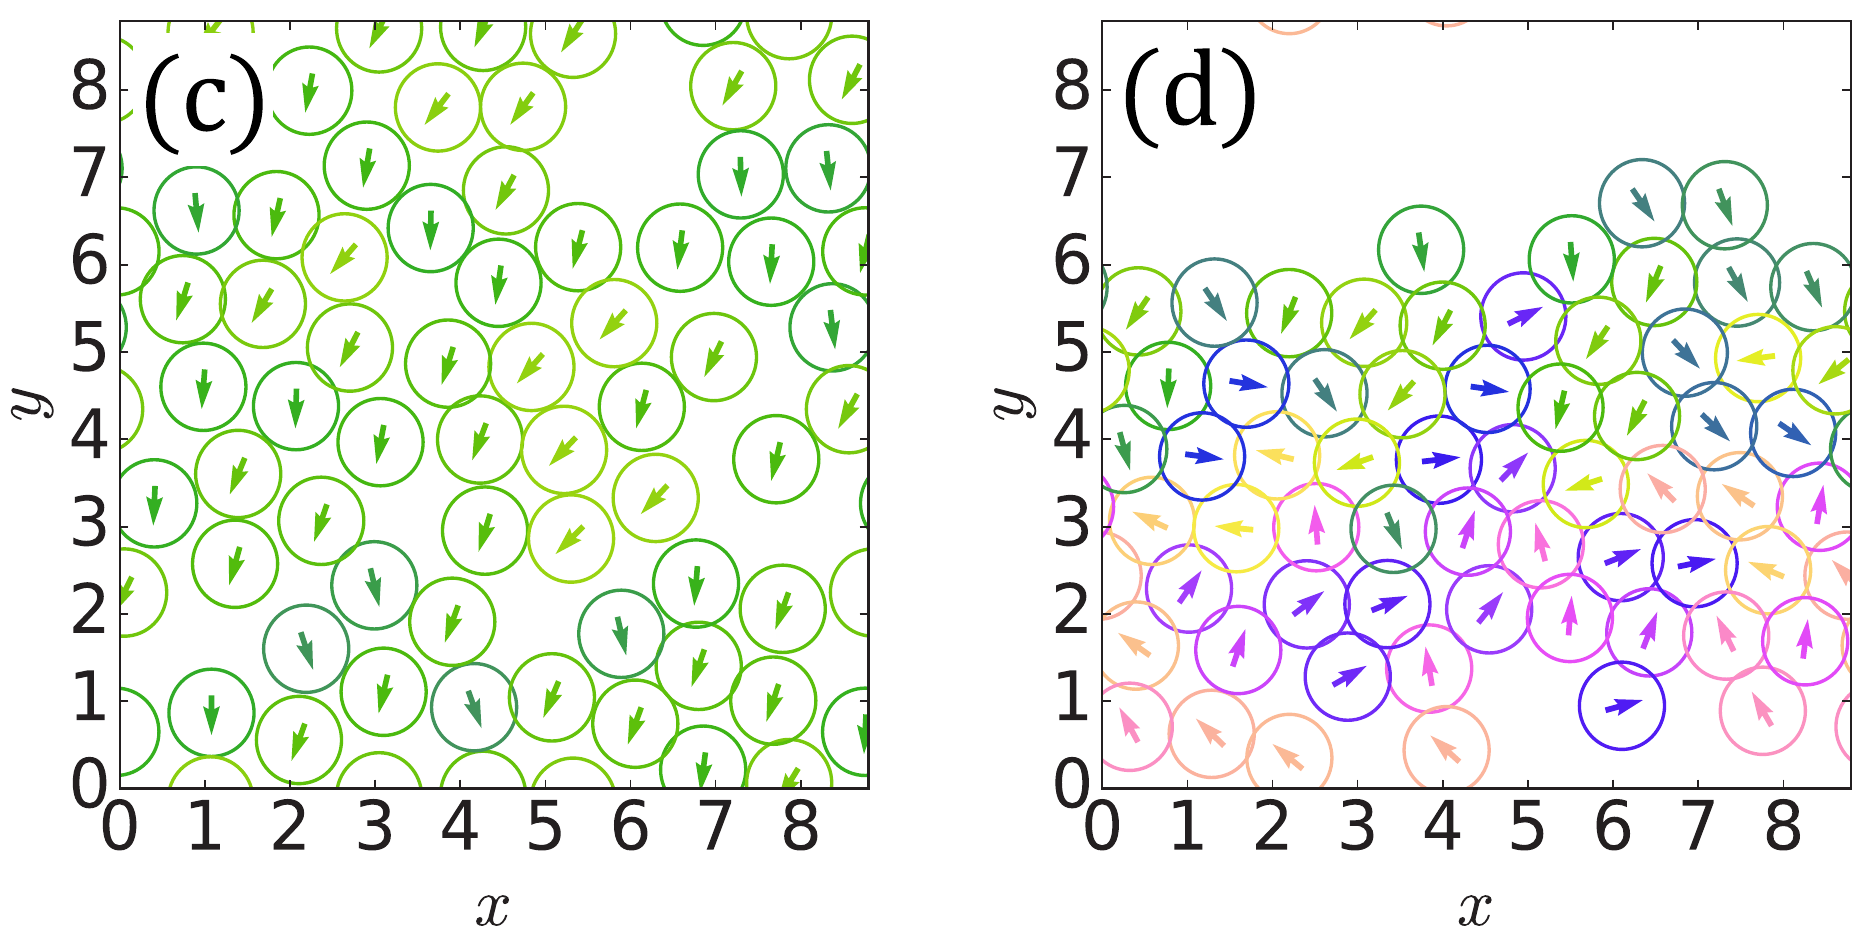
\includegraphics[width=0.88\linewidth]{Nemoto_2019_Fig1cd.png}
\captionof{figure}{Snapshots (Ref.~\cite{nemoto2019optimizing}, Fig.~1(c,d)) in the collective motion (CM) and phase separated arrested (PSA) phases. Arrows and colors encode the direction of self-propulsion.}
}
}

\blockA{Model and methods}{

\begin{multicols}{2}

\paragraph{Natural dynamics}

${\color{CaRed} N}$ ABPs in 2D, with diameters $\sigma$, positions $\bm{r}_i$ and orientations $\bm{u}_i \equiv (\cos\theta_i, \sin\theta_i)$, interacting via a WCA potential $U$, following
\begin{align*}
\dot{\bm{r}}_i & = v_0 \bm{u}_i -
D \nabla_i U
+ \sqrt{2D} \, \bm{\eta}_i \;\\
\dot{\theta}_i & = \sqrt{2 D_r} \, \xi_i
\end{align*}
with $\bm{\eta}_i$, $\xi_i$ Gaussian white noises, in a square box with periodic boundary conditions, at packing fraction ${\color{CaRed} \phi} = 0.65$. Ratio ${\color{CaRed} \tilde{l}_{\rm p}} = v_0/\sigma D_r$ is the scaled persistence length.\\

\paragraph{Orientational order parameter}

An \textbf{orientational order parameter} (polarisation) quantifies collective motion
\begin{align*}
\bm{\nu} = \frac{1}{N} \sum_{i=1}^N \bm{u}_i,~ \nu = |\bm{\nu}|,~ \bar{\nu}_{\tau} = \frac{1}{\tau} \int_0^{\tau} \nu(t) \, \mathrm{d}t.\\
\end{align*}

\paragraph{Active work}

We use a dimensionless and normalised measure of the work of non-conservative self-propulsion forces
\begin{align*}
w_\tau = &~\frac{1}{v_0 N\tau} \sum_{i=1}^N \int_0^\tau \bm{u}_i \circ \mathrm{d}\bm{r}_i%\\
% = &~1\\
% &~- \frac{D}{v_0 N \tau} \sum_i \int_0^{\tau} \bm{u}_i \cdot \nabla_i U \, \mathrm{d}t &&\Big\} w_{f, \tau}\\
% &~+ \frac{1}{v_0 N \tau} \sum_i \int_0^{\tau} \bm{u}_i \circ \sqrt{2 D} \bm{\eta}_i \, \mathrm{d}t &&\Big\} w_{\eta, \tau}
\end{align*}
called \textbf{active work}, illustrated thereafter.

\vfill\null
\columnbreak
\paragraph{Biased ensemble}

Active work $w_{\tau}$ satisfies a \textbf{large deviation principle} in the limit of large $\tau$
\begin{align*}
P(w_{\tau}) \asymp \exp[-\tau N I(w_{\tau})]
\end{align*}
where $I(w_{\tau})$ is a scaled \textbf{rate function}, which is related to the scaled cumulant generating function
\begin{align*}
\psi(s) = \lim_{\tau \to \infty} \frac{1}{N \tau} \log \left\langle \exp\left(- s N \tau w_{\tau} \right) \right\rangle
\end{align*}
via Legendre transform, where $s$ is the \textbf{biasing parameter}. A Boltzmann-like distribution of trajectories is defined, with respect to which the \textbf{biased average} of an observable $\mathcal{A}$ is
\begin{align*}
\left\langle\mathcal{A}\right\rangle_s = \frac{\left\langle\mathcal{A} \, e^{-s N \tau w_{\tau}}\right\rangle}{\left\langle e^{-s N \tau w_{\tau}} \right\rangle}
\end{align*}
and is computed numerically with a \textbf{cloning algorithm}.\\

% Biased average of the active work of a free particle is computed
% \begin{align*}
% w^{\rm free}(s) = 1 - \frac{2 s D}{v_0^2}
% \end{align*}
% showing that the biasing effectively rescales the self-propulsion velocity via the $w_{\eta, \tau}$ term.\\

\hrule
\mbox{}\\

\begin{minipage}{0.49\linewidth}
\centering
\bf Flocking
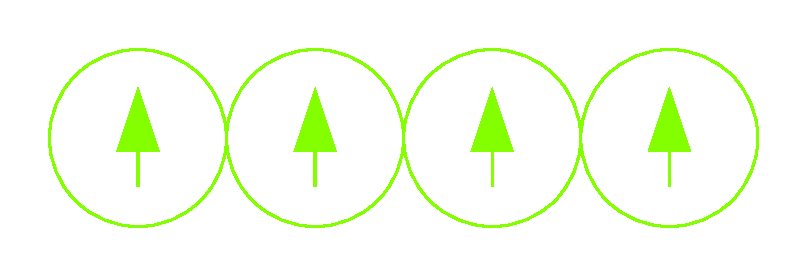
\includegraphics[width=\linewidth]{w1.eps}
$\bm{u}_i \cdot \nabla_i U = 0$\\
$w_{\tau} \approx 1, \nu = 1$
\end{minipage}
\hfill
\begin{minipage}{0.49\linewidth}
\centering
\bf Jamming
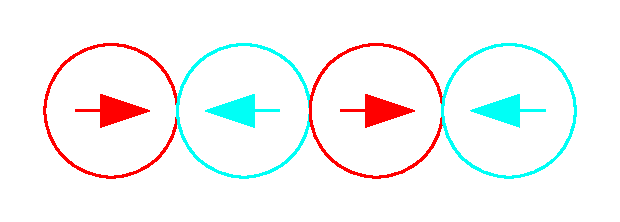
\includegraphics[width=\linewidth]{w0.eps}
$\dot{\bm{r}}_i \approx 0$\\
$w_{\tau} \approx 0, \nu = 0$
\end{minipage}

\end{multicols}

}

\blockA{Transition to collective motion}
{
\begin{itemize}
  \item \textbf{Dynamical phase transition} between an isotropic ($\langle \bar{\nu}_{\tau} \rangle_s = \mathcal{O}(1/N)$) and a CM state ($\langle \bar{\nu}_{\tau} \rangle_s = \mathcal{O}(1)$) at $s^* \approx -D_r$, $\langle w_{\tau} \rangle_{s^*} = w^*$, denoted by the maximum in
  \begin{align*}
    -\partial_s \langle w_{\tau} \rangle_s = \partial^2_s \psi(s) = \lim_{\tau \to \infty} \tau N \mathrm{Var}(w_{\tau})_s.\\
  \end{align*}
\end{itemize}
{\centering
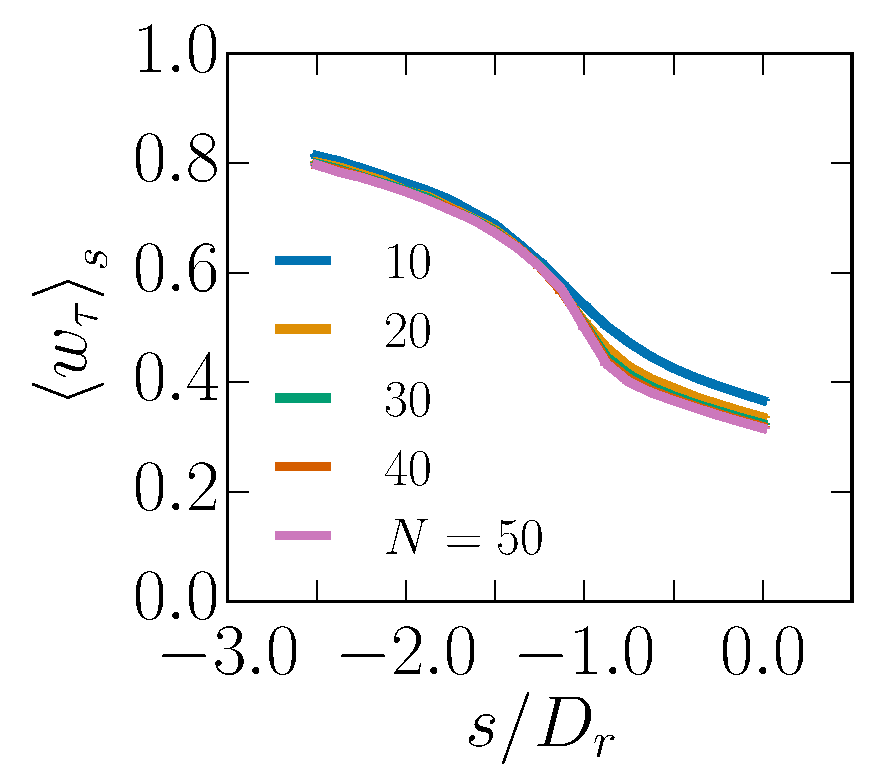
\includegraphics[width=0.40\linewidth]{sWork_Dk6500_Ll5000_To1000.eps}
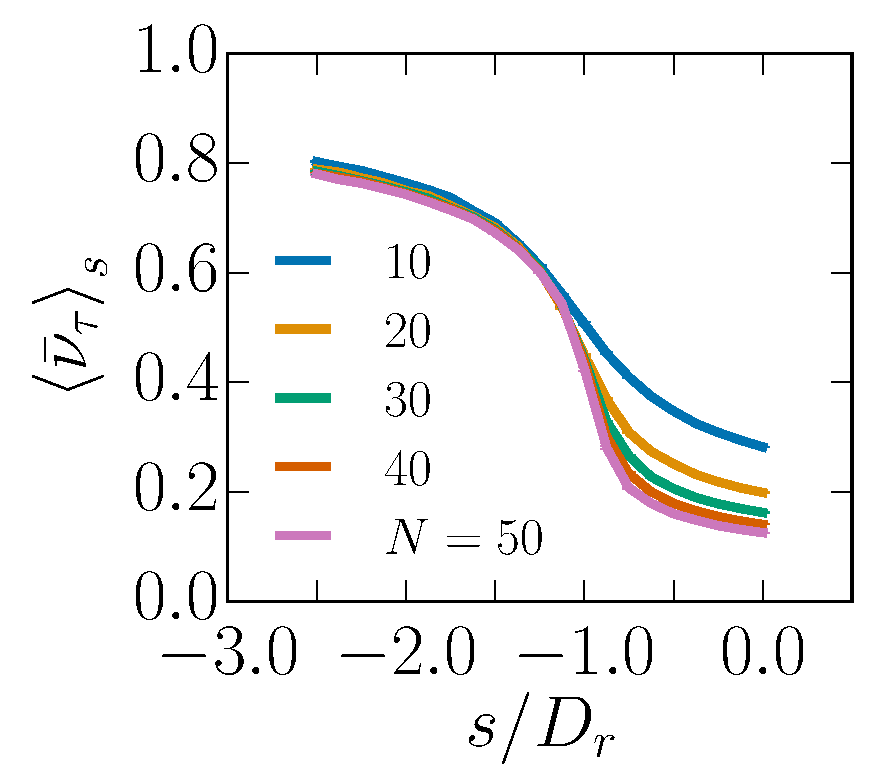
\includegraphics[width=0.40\linewidth]{sOrder_Dk6500_Ll5000_To1000.eps}
\captionof{figure}{Biased averages of the active work $\langle w_{\tau} \rangle_s$ and the orientational order parameter $\langle \bar{\nu}_{\tau} \rangle_s$ as functions of the biasing parameter $s$ at $\tilde{l}_{\rm p} = 5$.}
}

}

\column{0.5}

\blockA{Collective motion state}
{
\begin{multicols}{2}
\textbf{Modified orientational dynamics}
% \begin{align*}
% U^{\rm con}_g = - \frac{g N}{D_r} \nu^2
% \end{align*}
\begin{align*}
\dot{\theta}_i = - D_r \frac{\partial}{\partial \theta_i} \left(- \frac{g N}{D_r} \nu^2\right) + \sqrt{2 D_r} \xi_i
\end{align*}
give an \textbf{upper bound} to the rate function
\begin{align*}
I(\langle w_{\tau} \rangle^{\rm con}_g) \leq \lim_{\tau\to\infty} \frac{1}{N \tau} \left\langle \log P^{\rm con}_g/P \right\rangle^{\rm con}_g.
\end{align*}

\textbf{Contraction principle} gives a \textbf{lower bound} to the rate function
\begin{align*}
I(\langle w_{\tau} \rangle_s) \geq \mathcal{J}_1(\langle \bar{\nu}_{\tau} \rangle_s)
\end{align*}
from $\mathcal{J}_1$ the rate function of polarisation $\nu$.
\end{multicols}

\begin{itemize}
  \item In the CM state ($w > w^*$) both bounds perform well, showing that \textbf{fluctuations of $w_{\tau}$ are strongly coupled to those of $\bar{\nu}_{\tau}$}.
\end{itemize}

{\centering
\includegraphics[width=0.70\linewidth]{boundRate40.eps}
\captionof{figure}{Rate function $I(w)$ (orange) with upper bound from controlled dynamics (blue) and lower bound from the cloning of rotors (green). Inset shows the relative errors of these bounds to the rate function.}
}

}

\blockA{Hydrodynamic description}
{

Consider a \textbf{minimal top-down hydrodynamic description} of ABPs
\begin{align*}
&\dot{\rho} = - \nabla \cdot \left(v_0 \rho \bm{P} - D(\rho)\nabla\rho + \sqrt{2 \sigma(\rho)} \bm{\eta}\right),\\
&\dot{\bm{P}} = - \gamma(\rho, \bm{P}) f(\bm{P}) + b(\rho, \bm{P}) \nabla \rho + \sqrt{2 \gamma(\rho, \bm{P})} \bm{\xi}.
\end{align*}
% biased with respect to
% \begin{align*}
% N t w_t = \int_0^t \int_{[0, L]^2} \omega(\rho, \bm{P}) \, \mathrm{d}t \, \mathrm{d}^2\bm{r}.
% \end{align*}

\begin{multicols}{2}

\paragraph{Laudau theory}

Typical behaviour in the biased ensemble is obtained by \textbf{minimising the action}
\begin{align*}
{\cal S} = \frac{L^2}{D(\bar{\rho})} \left[ \bar\rho {\cal J}(\bm{P}) + s \bar\rho \left( \langle w_\tau\rangle + \frac{c_\omega}{2} | \bm{P} |^2 \right)\right]
\end{align*}
with $\mathcal{J}$ the rate function of polarisation $\bm{\nu}$.\\

\begin{itemize}
  \item It predicts a \textbf{spontaneous breaking of symmetry} at $s^* = -D_r/c_{\omega} \approx D_r$.\\
\end{itemize}

{
\centering
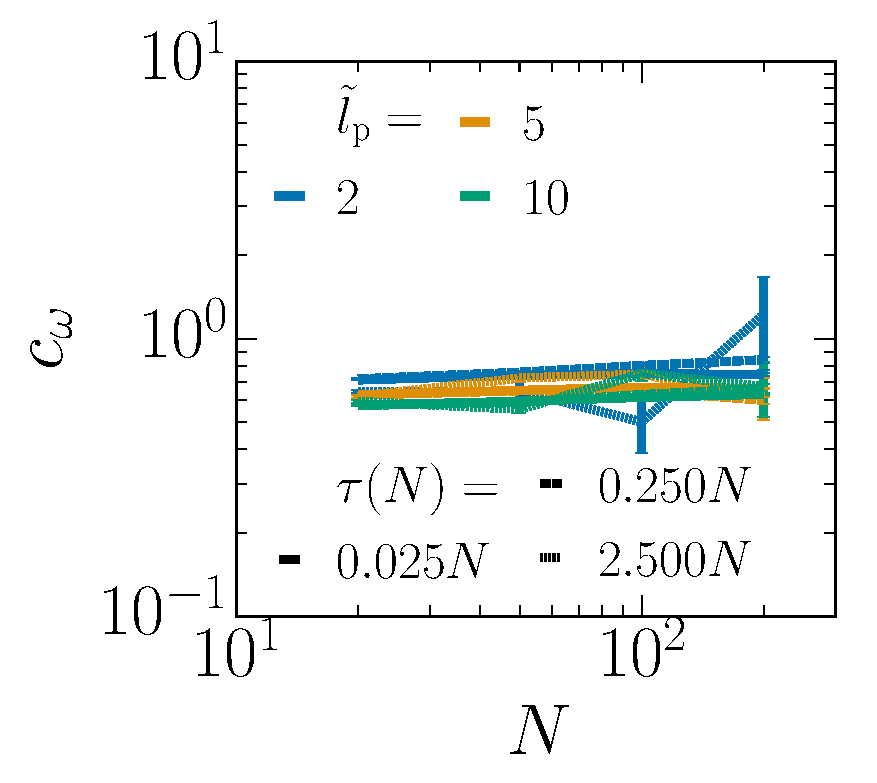
\includegraphics[width=0.8\linewidth]{covPW_Dk6500.eps}
\captionof{figure}{Covariance $c_{\omega} = \frac{  \bar \rho  \tau^2L^4  D_r^2}{2}  \mathrm{Cov}\left( w_{\tau}, |\bm{\nu}_{\tau}|^2\right)$.}
}

% \vfill\null
\columnbreak
\paragraph{Density fluctuations}

At $\bm{P} = 0$ it is equivalent to bias with respect to $|\tilde{\rho}_{\bm{q}}|^2$, and it follows
\begin{align*}
S_s(q) = \langle|\tilde{\rho}_{\bm{q}}|^2\rangle_s = \begin{cases} \chi_0, &s=0, \\ b_s q, &s < 0. \end{cases}\\
\end{align*}

\begin{itemize}
  \item In finite simulations, biasing results in a \textbf{suppression of density fluctuations}.\\
\end{itemize}

\vfill\null
{\centering

\includegraphics[width=0.8\linewidth]{S_Nn1000_Dk6500_Ll5000_NCo1000.eps}
\captionof{figure}{Biased structure factor at $\tilde{l}_{\rm p} = 5$ and $N = 100$.}
}

\end{multicols}

}

\blockB{Conclusions}
{
\begin{itemize}
  \item Spontaneous breaking of rotational symmetry happens at \textbf{finite biasing}, and is qualitatively understood through the introduction of \textbf{effective aligning interactions}.
  \item In the isotropic regime, enhanced active work is associated with \textbf{suppressed density fluctuations}.
\end{itemize}
}

\blockC{References}
{
\begin{refsection}
\nocite{*}
\printbibliography[heading=empty]
\end{refsection}
}

\blockBlank{
\begin{minipage}[c]{\linewidth}
\includegraphics[height=4cm]{umontpellier.eps}
\hfill

\includegraphics[height=4cm]{cnrs.eps}
\hfill

\includegraphics[height=3cm]{simons.eps}
\hfill
\includegraphics[height=4cm]{cambridge.eps}
\hfill

\includegraphics[height=4cm]{uparis.eps}
\end{minipage}
}

\end{columns}

\end{document}
